% -*- coding: UTF-8 -*-
% hurlex-chapt5.tex
% hurlex 开发文档 第5章内容

\section {相关库函数和调试打印函数}

\par 截至前四章,我们已经实现了一个能在屏幕上任意输出字符的小内核了。但是在开始新的探索之前,需要完成一些在内核开发中\allowbreak
至关重要的模块。

\subsection {C语言的字符串处理函数}

\par 我们之前多次提到现有的用户态的C语言标准库无法使用在内核中,但是内核开发中难免要用到诸如字符串操作的函数,所以\allowbreak
我们需要自己实现这些字符串相关的函数。

\par 首先给出函数的声明:

\begin{lstlisting}[language = C, label = include/string.h, caption = include/string.h]
#ifndef INCLUDE_STRING_H_
#define INCLUDE_STRING_H_

#include "types.h"

void memcpy(uint8_t *dest, const uint8_t *src, uint32_t len);

void memset(void *dest, uint8_t val, uint32_t len);

void bzero(void *dest, uint32_t len);

int strcmp(const char *str1, const char *str2);

char *strcpy(char *dest, const char *src);

char *strcat(char *dest, const char *src);

int strlen(const char *src);

#endif 	// INCLUDE_STRING_H_
\end{lstlisting}

\par 至于函数的实现我只给出其中几个函数的参考实现,剩下的请大家自己实现吧,考验大家C语言指针基本功的时候到了。\allowbreak
\footnote{友情提醒,这里的函数最好在用户态下进行编码和测试,确认正确无误了再放入内核中使用。}

\begin{lstlisting}[language = C, label = libs/string.c, caption = libs/string.c]
#include "string.h"

inline void memcpy(uint8_t *dest, const uint8_t *src, uint32_t len)
{
	for (; len != 0; len--) {
		*dest++ = *src++;
	}
}

inline void memset(void *dest, uint8_t val, uint32_t len)
{
	uint8_t *dst = (uint8_t *)dest;

	for ( ; len != 0; len--) {
		*dst++ = val;
	}
}

inline void bzero(void *dest, uint32_t len)
{
	memset(dest, 0, len);
}
\end{lstlisting}

\subsection {内核级的屏幕打印函数}

\par 初学C语言时使用的printf函数想必大家都很熟悉吧?可是在这里是没有办法使用现有的库的。不过完成了屏幕的控制输出之后,\allowbreak
我们就可以基于它同时根据printf函数的实现原理,写出一个内核态下可以进行屏幕打印的函数printk了。但是这里恐怕不敢展开来讲,\allowbreak
这涉及到C语言的可变形参表\footnote{也有译作"变长参数"或"可变参数列表"的。}和函数调用栈等繁多细节。原本我只想给出具体的\allowbreak
实现以供大家参考,但是又觉得带给大家"夹生饭"的做法不太好。所以我简单的结合代码给大家阐述下基本的实现原理,同时希望没理解\allowbreak
的读者自行检索相关资料,争取理解这个函数的实现。

\par 我们之前已经实现过了屏幕打印字符串和数字等内容的函数了,那么此时想实现printf函数,难点就在于构造这个最终打印的字符串。\allowbreak
现在摆在我们面前的问题其实只有两个,那就是如何知道有多少个参数传进来和如何知道每一个参数的类型。其实我们完全可以照搬printf\allowbreak
的做法,提供同样的接口。printf的用法大家很清楚,首先是一个待显示的字符串,里面分别用\%加相关字母的方式一一指明了后面的参数\allowbreak
数量和类型。只要我们传递正确的带有格式描述的字符串和相关参数,printf函数就能正确的打印出来结果。

\par 我们的printk函数的实现完全模仿printf函数的接口,首先是函数声明:

\begin{lstlisting}[language = C, label = include/debug.h, caption = include/debug.h]
#include "console.h"
#include "vargs.h"

// 内核的打印函数
void printk(const char *format, ...);

// 内核的打印函数 带颜色
void printk_color(real_color_t back, real_color_t fore, const char *format, ...);
\end{lstlisting}

\par 后面一个printk\_color对应之前的带颜色的屏幕输出,因为C语言没有C++那样的函数重载或者默认参数的特性,所以我们只能定义\allowbreak
两个函数了。printk函数的声明的参数列表首先是一个字符串,然后是三个小数点,这样的话编译器会允许我们在调用printk函数的时候\allowbreak
带有任意多个实参了。剩下的问题就是在printk的实现里,如何在没有形参名的情况下找到取到每一个参数。解决了这个问题之后,我想\allowbreak
剩下的问题就很简单了。

\par 我们先贴出另一个所需要的头文件 vargs.h 的内容:

\begin{lstlisting}[language = C, label = include/vargs.h, caption = include/vargs.h]
#ifndef INCLUDE_VARGS_H_
#define INCLUDE_VARGS_H_

typedef __builtin_va_list va_list;

#define va_start(ap, last)         (__builtin_va_start(ap, last))
#define va_arg(ap, type)           (__builtin_va_arg(ap, type))
#define va_end(ap) 

#endif 	// INCLUDE_VARGS_H_
\end{lstlisting}

\par 我们定义了几个宏,这几个宏用于取得每一个调用printk函数时传入的参数值。可能你会很诧异va\_list、\_\_builtin\_va\_start和\allowbreak
\_\_builtin\_va\_arg这几个类似于函数东西在何处定义,其实它们是gcc内置的变量和函数之类的存在了。GNU C提供了很多扩展,这\allowbreak
只是其中的一个。而其他平台上通常把它们定义为宏,下面是一个简化版的定义:\allowbreak
\footnote{注意这里是简化版的定义,事实上出于x86压栈元素长度的限制和优化的考虑,小于等于4字节的类型统一扩展到4字节压栈。大于\allowbreak
4字节小于等于8字节的类型统一以8字节压栈(另外32位压栈指令的操作数只能是16位或者32位的)。}

\begin{lstlisting}[language = C, label = 可变形参表, caption = 可变形参表]
#define  va_list              char *

#define  va_start(p, first)   (p = (va_list)&first + sizeof(first))
#define  va_arg(p, next)      (*(next*)((p += sizeof(next) ) - sizeof(next)))
#define  va_end(p)            (p = (va_list)NULL)
\end{lstlisting}

\par 我们可以看到,这几个宏的作用是根据第一个参数的地址和类型,通过逐渐计算出以后每一个参数的起始地址的方法取出每一个参数。\allowbreak
也就是说这是建立在"函数调用的参数在内存里是连续的"这一简单假设之上的。

\par 我们知道函数调用是通过栈来传递参数的,那参数按照什么顺序入栈?入栈后使用完参数后何处的代码清理之前栈里的参数呢?\allowbreak
事实上传递参数的工作必须由函数调用者和函数本身来协调,即就是所谓的"调用约定"。现行的调用约定有很多中,而C语言默认的\allowbreak
调用约定就是cdecl了,cdecl约定规定由调用者从右向左向栈里连续的压入参数,在函数返回之后,再清理掉压入的参数以保证堆栈平衡。\allowbreak
对于类似于 func(1, 2, 3, 4); 这样的函数调用编译后生成的汇编代码类似下面这样:

\begin{lstlisting}[language = {[x86masm]Assembler}, label = 函数调用, caption = 函数调用]
	push 4
	push 3
	push 2
	push 1
	call func
	sub esp, 16
\end{lstlisting}

\par 大家看明白没有?默认情况下按照cdecl约定,参数被从右向左连续压栈了,而且调用完后根据参数长度自行清理了参数。\allowbreak
\footnote{当然C语言中调用处理这一步是编译器自动生成的,明白了原理之后我们只要实现具体的函数即可。}明白了这些,我们\allowbreak
就为以后的汇编和C语言函数的相互调用打好了基础。而且也明白了参数在栈里面是连续的存储的,只要知道了第一个参数\allowbreak
在栈里的地址和每个参数的类型,就能计算出每一个参数的地址访问到它们了。

\par printk涉及的代码比较多,没有办法在这里一一细说了。还是那句话,需要大家主动的去探索学习。这个项目使用的printk\allowbreak
甚至直接参考和复制了Linux早期内核里的一些思想和子函数的实现,希望大家自己去研究一下。至于使用的方法就很简单了,\allowbreak
它和大家熟悉的printk函数没有什么太大差异。

\subsection{代码级调试的实现}

\par 不知道大家之前的编码过程是否顺利?是否遇到了运行后无法得出结果的问题?我们平时构建用户级程序的时候,有很长一段\allowbreak
都是在调试。那这个小内核能否像平时那样轻松的调试查错?如果不能或者只能进行汇编级别的调试,恐怕会对我们的后期开发造成\allowbreak
很大的影响。毕竟在客观上bug一就避免不了,那我们能否使用平日里习惯的调试工具进行轻松的排错?答案是肯定的。我们给出的\allowbreak
解决方案就是使用qemu联合gdb进行C语言源代码级别的调试。具体怎么做呢?

\par 首先是通讯问题,因为qemu和gdb运行的时候毕竟是两个进程,数据交换必然涉及到进程间通信机制。所幸它们都支持一个标准的\allowbreak
调试协议,而且开启的方法都很简单。qemu使用以下命令启动即可:

\begin{Verbatim}[frame=single]
  qemu -S -s -fda floppy.img -boot a 
\end{Verbatim}

\par 这几个参数中 -fda floppy.img 和 -boot a 是指定启动的镜像,-s 这个参数指的是启动时开启1234端口等待gdb连接\allowbreak
(这个参数从字面上看比较隐晦),-S 是指是启动时不自动开始运行,等待调试器的执行命令。以调试模式启动了虚拟机之后,再\allowbreak
启动gdb。需要注意的是,此时的gdb没有内核程序的符号文件,没有办法进行代码级调试。解决的办法很简单,我们使用命令\allowbreak
加载待调试内核对应的可执行文件即可。\footnote{别忘了我们的Makefile中的编译参数中指明了生成内核的调试信息。}\allowbreak
启动了gdb之后,我们依次执行以下指令即可。

\begin{Verbatim}[frame=single]
  file hx_kernel
  target remote :1234
  break kern_entry
  c
\end{Verbatim}

\par 这几个命令的意思分别是加载待调试文件的符号信息;连接本地的1234端口;在 kern\_entry 函数处下断点;执行到断点处。\allowbreak
\footnote{之前修改过Makefile中生成的内核文件名的读者们注意这里必须和实际的内核文件名保持一致。}\allowbreak
如果每次调试都需要这样做的话也未免太麻烦了,所以我们可以把上面几条命令写在scripts目录里的gdbinit文件里,在启动gdb\allowbreak
的时候自动加载执行。甚至在Makefile里也有我写的一个专门用于调试的伪目标debug 。在开始测试前,先给出我此时的目录结构以便\allowbreak
大家核对。

\begin{Verbatim}[frame=single]
.
|-- boot
|   `-- boot.s
|-- drivers
|   `-- console.c
|-- floppy.img
|-- include
|   |-- common.h
|   |-- console.h
|   |-- debug.h
|   |-- string.h
|   |-- types.h
|   `-- vargs.h
|-- init
|   `-- entry.c
|-- kernel
|   `-- debug
|       |-- debug.c
|       `-- printk.c
|-- libs
|   |-- common.c
|   `-- string.c
|-- Makefile
`-- scripts
    |-- gdbinit
    `-- kernel.ld
    
    8 directories, 17 files
\end{Verbatim}

\par 现在开始调试测试,执行以下命令开始调试。\footnote{我使用的是cgdb,这是一个给gdb提供了代码高亮显示的前端,你可以安装它或者\allowbreak
修改Makefile里面debug项目下的 cgdb -x scripts/gdbinit 为 gdb -tui -x scripts/gdbinit}

\begin{Verbatim}[frame=single]
  make
  make debug
\end{Verbatim}

\par 源码级的调试效果如图:

\begin{figure}[ht]
      \centering
      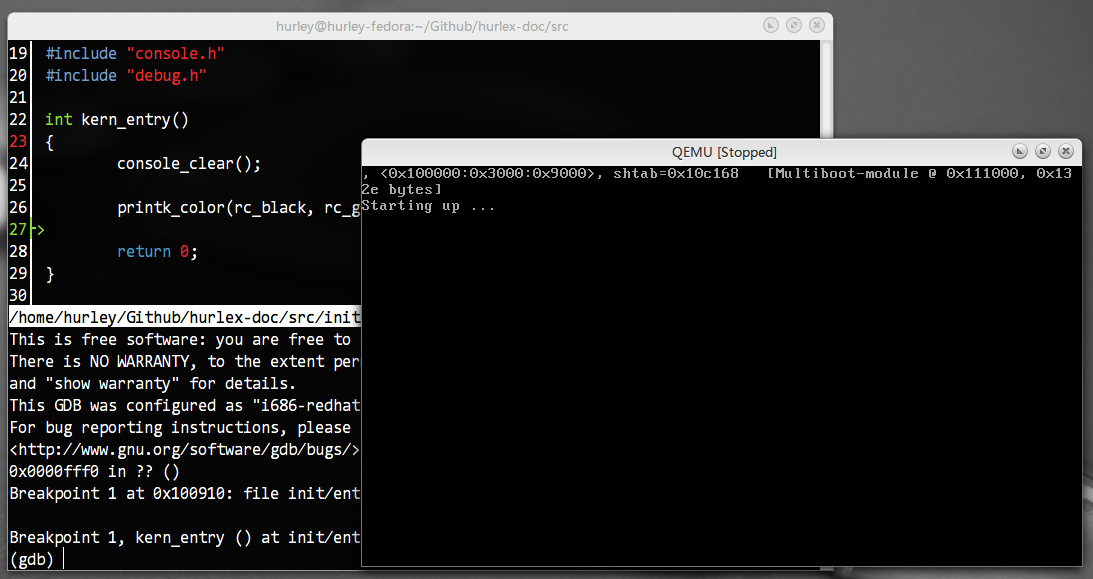
\includegraphics[scale=0.4]{picture/chapt5/os_debug.png}
      \caption{源码级别调试内核}
\end{figure}

\par 剩下的调试操作和平时使用gdb的方法别无二致,所以大家应该都不陌生。有的读者可能需要学习一些查看寄存器值之类的命令,请查阅手册吧。

\subsection{打印函数调用栈}

\par 解决了代码级调试的功能,我们来完成一些稍微复杂的函数,那就是当内核遇到致命错误时,如何自动打印当前的函数调用栈?\allowbreak
这涉及到GRUB Multiboot规范的很多细节和函数调用栈的结构。我们先从Multiboot的细节说起。

\par 在boot/boot.s里的start函数调用kern\_entry函数之前,我们把ebx寄存器的值赋给了一个全局变量glb\_mboot\_ptr。这是一个指向了\allowbreak
multiboot\_t类型结构体的指针,这个结构体存储了GRUB在调用内核前获取的硬件信息和内核文件本身的一些信息。我们先给出具体\allowbreak
的结构体的定义如下:

\begin{lstlisting}[language = C, label = include/multiboot.h, caption = include/multiboot.h]
#ifndef INCLUDE_MULTIBOOT_H_
#define INCLUDE_MULTIBOOT_H_

#include "types.h"

typedef
struct multiboot_t {
	uint32_t flags;		// Multiboot 的版本信息
	/** 
	 * 从 BIOS 获知的可用内存
	 *
	 * mem_lower 和 mem_upper 分别指出了低端和高端内存的大小,单位是K。
	 * 低端内存的首地址是 0 ,高端内存的首地址是 1M 。
	 * 低端内存的最大可能值是 640K 
	 * 高端内存的最大可能值是最大值减去 1M 。但并不保证是这个值。
	 */
	uint32_t mem_lower;
	uint32_t mem_upper;

	uint32_t boot_device;	// 指出引导程序从哪个BIOS磁盘设备载入的OS映像
	uint32_t cmdline;	// 内核命令行
	uint32_t mods_count;	// boot 模块列表
	uint32_t mods_addr;
	
	/**
	 * ELF 格式内核映像的 section 头表。包括每项的大小、一共有几项以及作为名字索引
	 * 的字符串。
	 */
	uint32_t num;
	uint32_t size;
	uint32_t addr;
	uint32_t shndx;

	/**
	 * 以下两项指出保存由BIOS提供的内存分布的缓冲区的地址和长度
	 * mmap_addr 是缓冲区的地址, mmap_length 是缓冲区的总大小
	 * 缓冲区由一个或者多个下面的 mmap_entry_t 组成
	 */
	uint32_t mmap_length;		
	uint32_t mmap_addr;
	
	uint32_t drives_length; 	// 指出第一个驱动器结构的物理地址	
	uint32_t drives_addr; 		// 指出第一个驱动器这个结构的大小
	uint32_t config_table; 		// ROM 配置表
	uint32_t boot_loader_name; 	// boot loader 的名字
	uint32_t apm_table; 	    	// APM 表
	uint32_t vbe_control_info;
	uint32_t vbe_mode_info;
	uint32_t vbe_mode;
	uint32_t vbe_interface_seg;
	uint32_t vbe_interface_off;
	uint32_t vbe_interface_len;
} __attribute__((packed)) multiboot_t;

/**
 * size 是相关结构的大小,单位是字节,它可能大于最小值 20
 * base_addr_low 是启动地址的低32位,base_addr_high 是高 32 位,启动地址总共有 64 位
 * length_low 是内存区域大小的低32位,length_high 是内存区域大小的高 32 位,总共是 64 位
 * type 是相应地址区间的类型,1 代表可用 RAM,所有其它的值代表保留区域
 */
typedef
struct mmap_entry_t {
	uint32_t size; 		// size 是不含 size 自身变量的大小
	uint32_t base_addr_low;
	uint32_t base_addr_high;
	uint32_t length_low;
	uint32_t length_high;
	uint32_t type;
} __attribute__((packed)) mmap_entry_t;

// 声明全局的 multiboot_t * 指针
extern multiboot_t *glb_mboot_ptr;

#endif 	// INCLUDE_MULTIBOOT_H_
\end{lstlisting}

\par 结构体中有很多注释,大家结合具体的协议文档很容易就可以看懂。我们暂时需要关心的主要是符号表,其它的信息我们之后\allowbreak
用到的时候再讨论。也就是说,我们暂时只关注结构体中以下几个字段的内容即可:

\begin{lstlisting}[language = C, label = include/multiboot.h, caption = include/multiboot.h]
	......
	/**
	 * ELF 格式内核映像的 section 头表。
	 * 包括每项的大小、一共有几项以及作为名字索引的字符串表。
	 */
	uint32_t num;
	uint32_t size;
	uint32_t addr;
	uint32_t shndx;
	......
\end{lstlisting}

要理解下面的内容还真有些困难,因为它涉及的面太广了。我们先以ELF的文件格式做为切入点。我们先添加\allowbreak
elf.h这个头文件:

\begin{lstlisting}[language = C, label = include/elf.h, caption = include/elf.h]
#ifndef INCLUDE_ELF_H_
#define INCLUDE_ELF_H_

#include "types.h"
#include "multiboot.h"

#define ELF32_ST_TYPE(i) ((i)&0xf)

// ELF 格式区段头
typedef
struct elf_section_header_t {
  uint32_t name;
  uint32_t type;
  uint32_t flags;
  uint32_t addr;
  uint32_t offset;
  uint32_t size;
  uint32_t link;
  uint32_t info;
  uint32_t addralign;
  uint32_t entsize;
} __attribute__((packed)) elf_section_header_t;

// ELF 格式符号
typedef
struct elf_symbol_t {
  uint32_t name;
  uint32_t value;
  uint32_t size;
  uint8_t  info;
  uint8_t  other;
  uint16_t shndx;
} __attribute__((packed)) elf_symbol_t;

// ELF 信息
typedef
struct elf_t {
  elf_symbol_t *symtab;
  uint32_t      symtabsz;
  const char   *strtab;
  uint32_t      strtabsz;
} elf_t;

// 从 multiboot_t 结构获取ELF信息
elf_t elf_from_multiboot(multiboot_t *mb);

// 查看ELF的符号信息
const char *elf_lookup_symbol(uint32_t addr, elf_t *elf);

#endif 	// INCLUDE_ELF_H_
\end{lstlisting}

\par 这段结构体定义里包含了ELF文件的区段头、符号表等信息。我们给出从multiboot\_t结构中提取出ELF相关信息的代码:

\begin{lstlisting}[language = C, label = kernel/debug/elf.c, caption = kernel/debug/elf.c]
#include "common.h"
#include "string.h"
#include "elf.h"

// 从 multiboot_t 结构获取ELF信息
elf_t elf_from_multiboot(multiboot_t *mb)
{
	int i;
	elf_t elf;
	elf_section_header_t *sh = (elf_section_header_t *)mb->addr;

	uint32_t shstrtab = sh[mb->shndx].addr;
	for (i = 0; i < mb->num; i++) {
		const char *name = (const char *)(shstrtab + sh[i].name);
		// 在 GRUB 提供的 multiboot 信息中寻找
		// 内核 ELF 格式所提取的字符串表和符号表
		if (strcmp(name, ".strtab") == 0) {
			elf.strtab = (const char *)sh[i].addr;
			elf.strtabsz = sh[i].size;
		}
		if (strcmp(name, ".symtab") == 0) {
			elf.symtab = (elf_symbol_t*)sh[i].addr;
			elf.symtabsz = sh[i].size;
		}
	}

	return elf;
}

// 查看ELF的符号信息
const char *elf_lookup_symbol(uint32_t addr, elf_t *elf)
{
	int i;

	for (i = 0; i < (elf->symtabsz / sizeof(elf_symbol_t)); i++) {
		if (ELF32_ST_TYPE(elf->symtab[i].info) != 0x2) {
		      continue;
		}
		// 通过函数调用地址查到函数的名字
		if ( (addr >= elf->symtab[i].value) && (addr < (elf->symtab[i].value + elf->symtab[i].size)) ) {
			return (const char *)((uint32_t)elf->strtab + elf->symtab[i].name);
		}
	}

	return NULL;
}
\end{lstlisting}

\par 我们之前多次提过GRUB在载入内核之后,会读取ELF并把相关的信息\allowbreak
组织成结构体放在multiboot\_t结构,并把结构体指针放在ebx寄存器里传递给内核。其multiboot\_t结构的addr成员便指向的是\allowbreak
elf\_section\_header\_t类型的结构体数组,num成员是这个结构体数组的成员个数。

\par 这里的代码可能让大家一下子有点蒙,如果你觉得无从下手的话不妨在纸上画一画这几个结构体的关系图,这能帮助你理解。\allowbreak
对于这里的代码大家不必过于深究,毕竟ELF格式只是Linux平台下的一种可执行格式,而本文档的目的是想让大家建立对项目的\allowbreak
整体把握,细节问题就留给大家自己去理解吧。

\par 通过以上的努力,我们获取了ELF文件中关于每个函数的名称和它们代码的区域,那么此时如何使用这些信息寻找函数名称呢?\allowbreak
其实大家从elf\_lookup\_symbol函数的实现里就能看出来。我们提供了一个地址,然后查询这个地址在哪个函数的代码区间里,然后\allowbreak
返回了这个函数名的字符串指针。

\par 终于到了最后的函数调用栈问题了,这也是我们最终的打印调用栈函数panic的实现原理。

%\begin{lstlisting}[language = C, label = include/multiboot.h, caption = include/multiboot.h]
%\end{lstlisting}
